\documentclass[11pt,a4paper]{article}
\usepackage[utf8]{inputenc}
\usepackage[spanish]{babel}
\usepackage[pdftex]{graphicx}
\usepackage{color}
\usepackage{pdfpages}
\usepackage{url}

\title{Práctica Nagios}
\author{Nombre del estudiante que realiza el trabajo}
\date{Diciembre 2014}

\begin{document}

\maketitle
\tableofcontents
\clearpage

\section{Introducción a Nagios}

Aquí se debe introducir la definión de qué es Nagios\cite{web}. Sería deseable que introdujérais también 
otros sistemas similares a Nagios.

\section{Funcionamiento de Nagios}

Explicación de cómo funciona Nagios

Se pueden incluir figuras como por ejemplo la Figura~\ref{figura1} de la página \pageref{figura1}

\begin{figure}
\centerline{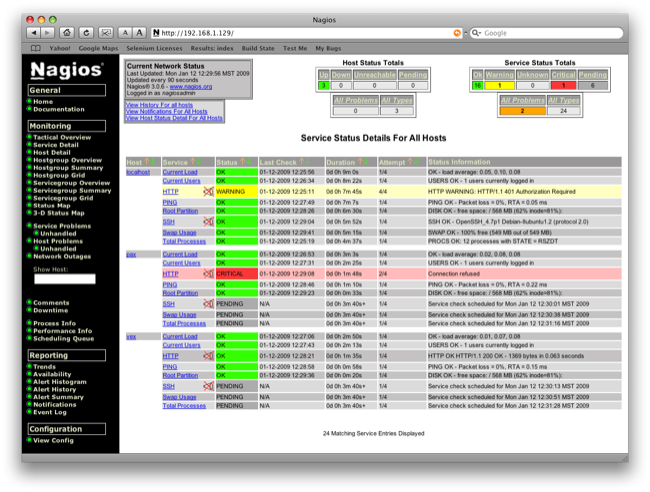
\includegraphics[width=6cm]{nagios3-1.png}}
\caption{Figura de ejemplo}
\label{figura1}
\end{figure}

\section{Instalación de Nagios}

En este apartado se explica cómo instalar Nagios de dos formas, desde repositorio y también compilando su código fuente. Ambos métodos tienen como distribución objetivo CentOs/RedHat.

\subsection{Instalación desde repositorio}

Suponiendo que se tiene acceso root a la máquina, el comando a ejecutar como superusuario es el siguiente

\begin{verbatim}
yum install nagios*
\end{verbatim}

esto se encargará de instalar Nagios, sus dependencias y los plugins. Los plugins nos permiten un mayor control de los sistemas a monitorizar así como una visualización más completa de la información.

\subsection{Instalación desde código fuente}

En primer lugar debemos crear el usuario y grupo al que pertenecerá la ejecución de Nagios. Esto se realiza con los siguientes comandos en modo superusuario

\begin{verbatim}
groupadd nagios
groupadd nagcmd
useradd nagios -g nagios
useradd nagios -g nagcmd
\end{verbatim}

El usuario Nagios será el que tendrá en ejecución el daemon correspondiente. Además hemos creado dos grupos, \textbf{nagios} y \textbf{nagcmd}

\begin{itemize}
\item \textbf{nagios}: El grupo principal de Nagios.
\item \textbf{nagcmd}: Este es el grupo que permite la ejecución de comandos externos a través de la interfaz web.
\end{itemize}

Ahora necesitamos instalar las dependencias, incluyendo el servidor web. De nuevo como superusuario ejecutamos lo siguiente

\begin{verbatim}
yum -y install httpd php glibc glibc-common gd gd-devel net-snmp
yum -y groupinstall "Development Tools"
\end{verbatim}

\textbf{httpd} y \textbf{php} serán los encargados del servidor web. \textbf{glibc}, \textbf{glibc-common}, \textbf{gd} y \textbf{gd-devel} son librerías para el manejo de gráficos y \textbf{net-snmp} es el que incluye las librerías para manejar el protocolo SNMP, que nos permitirá monitorizar los ordenadores en red.

\textbf{Development Tools} instala todos los paquetes necesarios para poder compilar los códigos fuente. Incluye, como pequeño ejemplo, gcc y make.

Ahora ya estamos listos para descargar el código fuente. En el momento de escribir esta memoria la última versión disponible es la 4.0.8 y es la que se usará a lo largo de la memoria, pero los pasos deberían ser iguales o muy similares en las versiones posteriores.

En primer lugar, descargamos y descomprimimos las fuentes de Nagios Core. Nagios Core es el engine que tiene toda la lógica de la aplicación, sobre él se añadirán plugins y demás para personalizarlo.

\begin{verbatim}
wget http://netcologne.dl.sourceforge.net/project/nagios/nagios-4.x/nagios-4.0.8/nagios-4.0.8.tar.gz
tar -xzf nagios-4.0.8.tar.gz
\end{verbatim}

Accedemos a la carpeta y realizamos un \textbf{./configure}

\begin{verbatim}
cd nagios-4.0.8
./configure
\end{verbatim}

\textbf{./configure} comprueba que las dependencias del programa estén satisfechas (por lo menos las esenciales). En caso de no cumplirse algún requisito indispensable el programa saldrá con un mensaje de error indicando qué se debe instalar. Si el programa considera que se cumplen los requisitos mínimos generará un fichero \textbf{Makefile} con los comandos necesarios para compilar e instalar el programa.

Una vez el comando ha acabado ejecutamos

\begin{verbatim}
make all
make install
make install-init
make install-commandmode
make install-config
make install-webconf
\end{verbatim}

\begin{itemize}
\item \textbf{all}: Compila el programa dejando los ejecutables preparados para ejecutarse desde local o para instalarse.
\item \textbf{install}: Copia los ejecutables base a sus respectivas carpetas para que se puedan encontrar desde el \$PATH.
\item \textbf{install-init}: Este comando instala el fichero en /etc/rc.d/init.d para poder iniciarlo y pararlo de manera cómoda.
\item \textbf{install-commandmode}: Instala y configura los permisos en el directorio para almacenar los ficheros externos de comandos.
\item \textbf{install-config}: Este comando instala plantillas de configuración en /usr/local/nagios/etc para que sea más fácil su edición.
\item \textbf{install-webconf}: Instala el fichero de configuración de Apache.
\end{itemize}

Ahora vamos a compilar e instalar los plugins desde código fuente, a fecha de escribir este artículo la última versión de los plugins es la 2.0.3

\begin{verbatim}
wget http://nagios-plugins.org/download/nagios-plugins-2.0.3.tar.gz
tar -xzf nagios-plugins-2.0.3.tar.gz
cd nagios-plugins-2.0.3
\end{verbatim}

Una vez descargados procedemos a su configuración, compilación e instalación.

\begin{verbatim}
./configure
make
make install
\end{verbatim}

Con esto tendríamos instalado Nagios y sus plugins desde código fuente, ahora sólo queda configurarlos. Esto se explica más adelante.

\section{Configurar Nagios}

Se debe explicar los distintos ficheros de configuración de Nagios y cómo se configuran para 
monitorizar tanto al sistema local como a sistemas remotos.

\section{Acceso a Nagios mediante el navegador}

Se debe explicar cómo se debe configurar el servidor web para acceder a Nagios a través del navegador
y  tambíen la interfaz web que presenta Nagios.

\section{Experiencia de instalación y configuración de  Nagios}

Se deben detallar los pasos que se han seguido para la instalación y configuración de Nagios
tanto para monitorizar el sistema local como sistemas remotos.

\begin{thebibliography}{1}

\bibitem{web} Página web del proyecto de Nagios: \url{http://www.nagios.org}

\end{thebibliography}

\end{document}
